\chapter{Spectral Analysis of Random Matrices}

Spectral analysis applied to adjacency matrices (and matrices derived from them, such as the Laplacian) provides a deep perspective on the macroscopic and topological properties of networks. By studying the eigenvalues and eigenvectors of these matrices, we can deduce crucial information about paths, the presence of cycles, network robustness, and the structure of hidden communities.

In the study of random networks, attention is primarily focused on three mathematical observables:
\begin{itemize}
    \item \textbf{Eigenvalue distribution}: to understand how the global energy or information of the network is distributed.
    \item \textbf{Maximum eigenvalue} (\( \lambda_{max} \)): strictly related to connectivity and diffusion limits on the network.
    \item \textbf{Nearest Neighbor Spacing Distribution} (NNSD): useful for identifying local correlations between the states of the network.
\end{itemize}

These spectral properties can be analyzed using tools from random matrix theory, which provides a framework for understanding the statistical properties of eigenvalues in large random matrices. By studying the spectral properties of random graphs, we can gain insights into the structure and dynamics of complex networks, and how they differ from more structured networks with community structure or other correlations. Our study cases will be:
\begin{itemize}
    \item Random symmetric matrix, with entries drawn from a Gaussian distribution, which can be used to model the adjacency matrix of an E-R random graph.
    \item E-R matrix, which is a specific case of a random symmetric matrix where the entries are binary (0 or 1) and represent the presence or absence of links between nodes in an E-R random graph.
    \item Hi-C matrix, which is a specific case of a random symmetric matrix that represents the contact frequencies between different regions of the genome in a Hi-C experiment. The spectral properties of Hi-C matrices can provide insights into the 3D organization of the genome and how it relates to gene regulation and other cellular processes.
\end{itemize}

% --------------------------------------------------------
\section{Gaussian Orthogonal Ensemble (GOE)}
% --------------------------------------------------------

\begin{definition}[Gaussian Orthogonal Ensemble]
    The Gaussian Orthogonal Ensemble (GOE) is one of the fundamental models in random matrix theory. It represents an ensemble of symmetric matrices where the independent elements (i.e., those on the diagonal and in the upper triangle) are random variables drawn from normal (Gaussian) distributions.
\end{definition}

This model is widely studied in physics and mathematics because its eigenvalue distribution has an explicit, symmetric form and can be calculated very efficiently. The term "orthogonal" derives from the fact that the statistical properties of these matrices remain invariant when subjected to orthogonal transformations.

\subsection{Wigner Semicircle Law}
For a random symmetric \( N \times N \) matrix whose elements are sampled from a Gaussian distribution \( \mathcal{N}(0, \sigma) \), the eigenvalue spectrum as \( N \to \infty \) follows the famous \textbf{Wigner semicircle law}.
\begin{figure}[H]
    \begin{minipage}{0.45\textwidth}
        \centering
        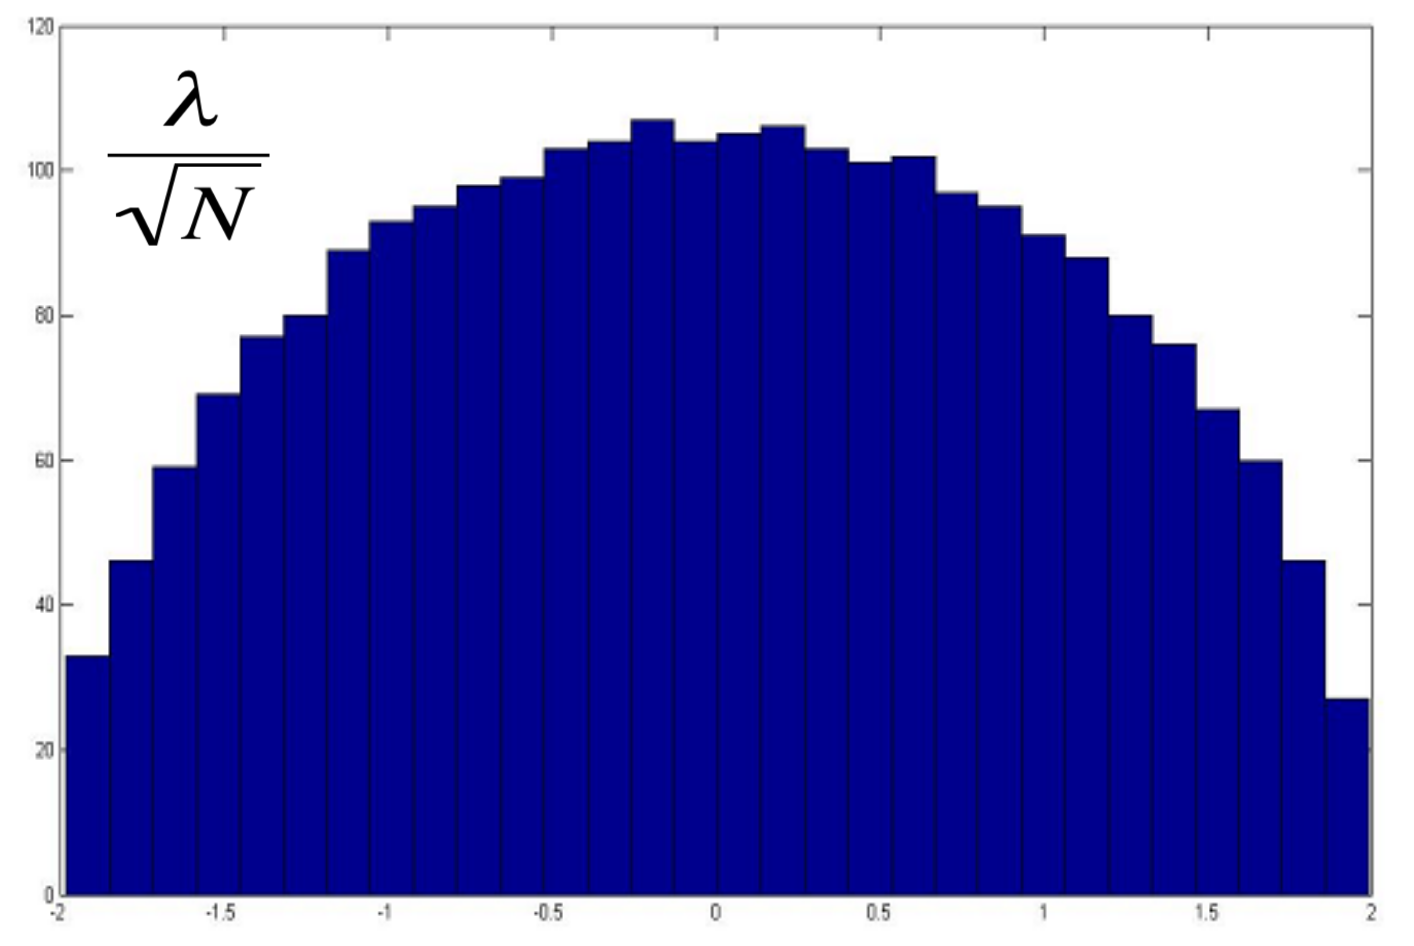
\includegraphics[width=0.9\textwidth]{img/wigner_semicircle.png}
        \caption{Eigenvalue spectrum of a GOE random matrix, showing the Wigner semicircle distribution.}
    \end{minipage}
    \hfill
    \begin{minipage}{0.5\textwidth}
        This means that the real eigenvalues tend to cluster together, forming a semicircle shape centered at the origin. The radius of this semicircle depends on the number of nodes \( N \) and the standard deviation \( \sigma \) of the original distribution:
        \[
            \lambda \in [-2\sigma\sqrt{N}, 2\sigma\sqrt{N}].
        \]
        The probability density function of the eigenvalues is defined as:
        \[
            \rho(\lambda) = \frac{\sqrt{4N\sigma^2 - \lambda^2}}{2\pi N\sigma^2}.
        \]
    \end{minipage}
\end{figure}

\subsection{Eigenvector Components}
In the GOE model, not only do the eigenvalues follow precise rules, but the components of the normalized eigenvectors are also distributed according to a Gaussian probability density. From a network science perspective, this implies that all eigenvectors are essentially delocalized and indistinguishable. They are therefore "uninformative" for finding hidden structures, as the Gaussian noise covers any pattern.

\begin{figure}[H]
    \begin{minipage}{0.55\textwidth}
        From the central limit theorem, if we have set of randomly distributed variables, their sum will tend to a Gaussian distribution, regardless of the original distribution of the variables. In the case of random graphs, the eigenvectors are linear combinations of the entries of the adjacency matrix, which are randomly distributed. Therefore, the components of the eigenvectors will also be randomly distributed and will tend to a Gaussian distribution due to the central limit theorem. This means that all eigenvectors will be equally distributed and will not provide any meaningful information about the structure of the graph, which is a key feature of random graphs.
    \end{minipage}
    \hfill
    \begin{minipage}{0.4\textwidth}
        \centering
        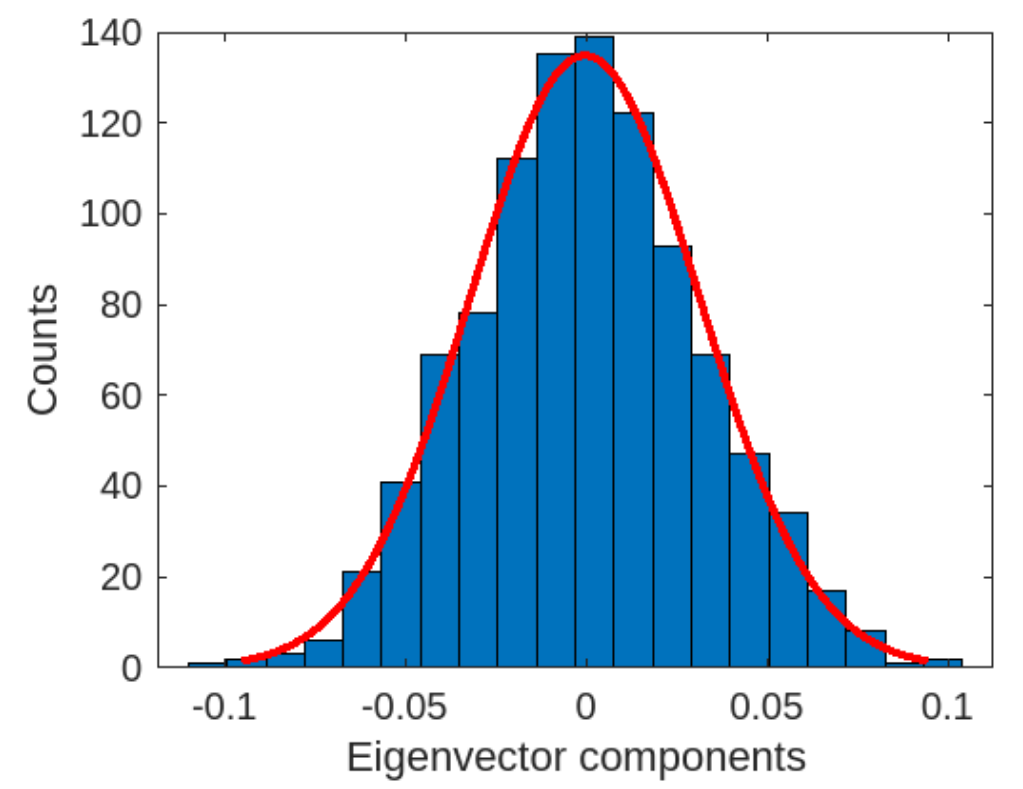
\includegraphics[width=0.9\textwidth]{img/gaussian-eigenvectors.png}
        \caption{Components of eigenvectors in a GOE random matrix, showing the Gaussian distribution.}
    \end{minipage}
\end{figure}

% --------------------------------------------------------
\section{Spectrum of Erdős-Rényi (E-R) Networks}
% --------------------------------------------------------

When we analyze the adjacency matrix associated with a connected, symmetric Erdős-Rényi (E-R) random network, we notice that the Wigner semicircle law approximately holds for the majority of the eigenvalues (the so-called "bulk"). However, the discrete nature of the connections (presence or absence of a link) brings out some specific topological characteristics.

\begin{remark}[E-R Spectrum and the Isolated Eigenvalue]
    The spectrum of an E-R network consists of the typical semicircular bulk (representing random topological noise) plus a single isolated principal eigenvalue (outlier), which distinctly detaches from the semicircle and scales linearly with \( N \).
    \begin{itemize}
        \item The standard deviation associated with the matrix is \( \sigma = \sqrt{N \cdot P(1-P)} \), where \( P \) is the connection probability.
        \item The isolated maximum eigenvalue can be approximated as \( \lambda_{max} \approx P \cdot N + 1 \).
    \end{itemize}
\end{remark}
The presence of this large eigenvalue is a key feature of E-R random graphs and distinguishes them from more structured networks, where there may be multiple large eigenvalues corresponding to different communities or other structures in the graph.

\begin{figure}[H]
    \begin{minipage}{0.55\textwidth}
        Furthermore note that:
        \[
            \mu\neq 0, \quad P = \frac{1}{N(N-1)}\sum_{ij} A_{ij},
        \]
        which means that the presence of a non-zero mean in the distribution of the matrix elements (i.e., a non-zero average degree in the graph) leads to the emergence of an isolated eigenvalue that scales with \( N \): the average degree introduces a global bias in the connectivity of the graph, which is reflected in the spectrum of its adjacency matrix.
    \end{minipage}
    \hfill
    \begin{minipage}{0.4\textwidth}
        \centering
        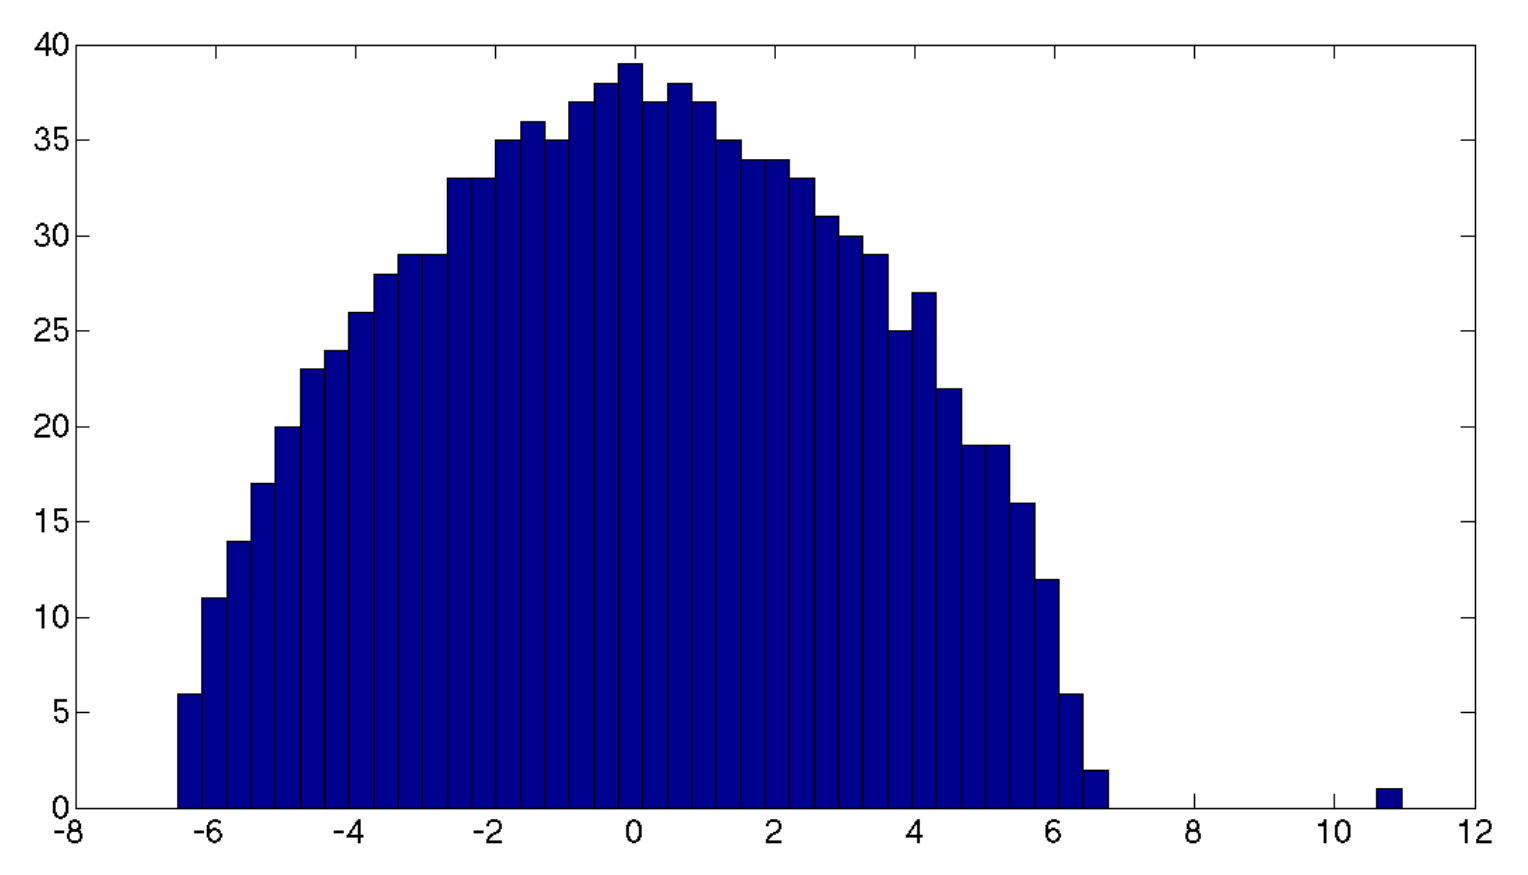
\includegraphics[width=0.9\textwidth]{img/E-R-spectrum.png}
        \caption{Eigenvalue spectrum of an E-R random graph, showing the semicircular bulk and the isolated maximum eigenvalue.}
    \end{minipage}
\end{figure}

As the system size \( N \) increases, the radius \(\sigma\) of the semicircle grows proportionally to \( \sqrt{N} \), while the maximum eigenvalue \( \lambda_{max} \) grows much faster, proportionally to \( N \). Consequently, the ratio between the radius and the maximum eigenvalue tends to zero. Macroscopically, the eigenvalue spectrum tends to converge towards that of a regular graph where all nodes possess the exact average connectivity \( \langle k \rangle \).

\subsubsection{Limits of the Maximum Eigenvalue \( \lambda_{max} \)}
By the Perron-Frobenius Theorem applied to non-negative matrices, the maximum eigenvalue of a network is unique and strictly tied to the node degrees. It is mathematically bounded by the average degree \( \langle k \rangle \) and the maximum degree \( k_{max} \) of the graph:
\[ \langle k \rangle \le \lambda_{max} \le k_{max} \]
This parameter is of fundamental importance in the study of dynamical processes on networks. For example, it governs the spreading rate of a virus in a contact network or defines the stability of synchronization among coupled oscillators.

\subsection{Directed Networks and the Circular Law}
When moving to directed (oriented) \( N \times N \) random matrices, symmetry is lost. As a result, the eigenvalues are no longer confined to the real number axis. Instead, they form a uniform circular distribution in the complex plane, known as the "Circular Law," with a radius of \( r = \sigma\sqrt{N} \). Even in a directed E-R network, we find this uniform distribution on the complex plane, almost always accompanied by the usual purely real and isolated eigenvalue.

\begin{figure}
    \centering
    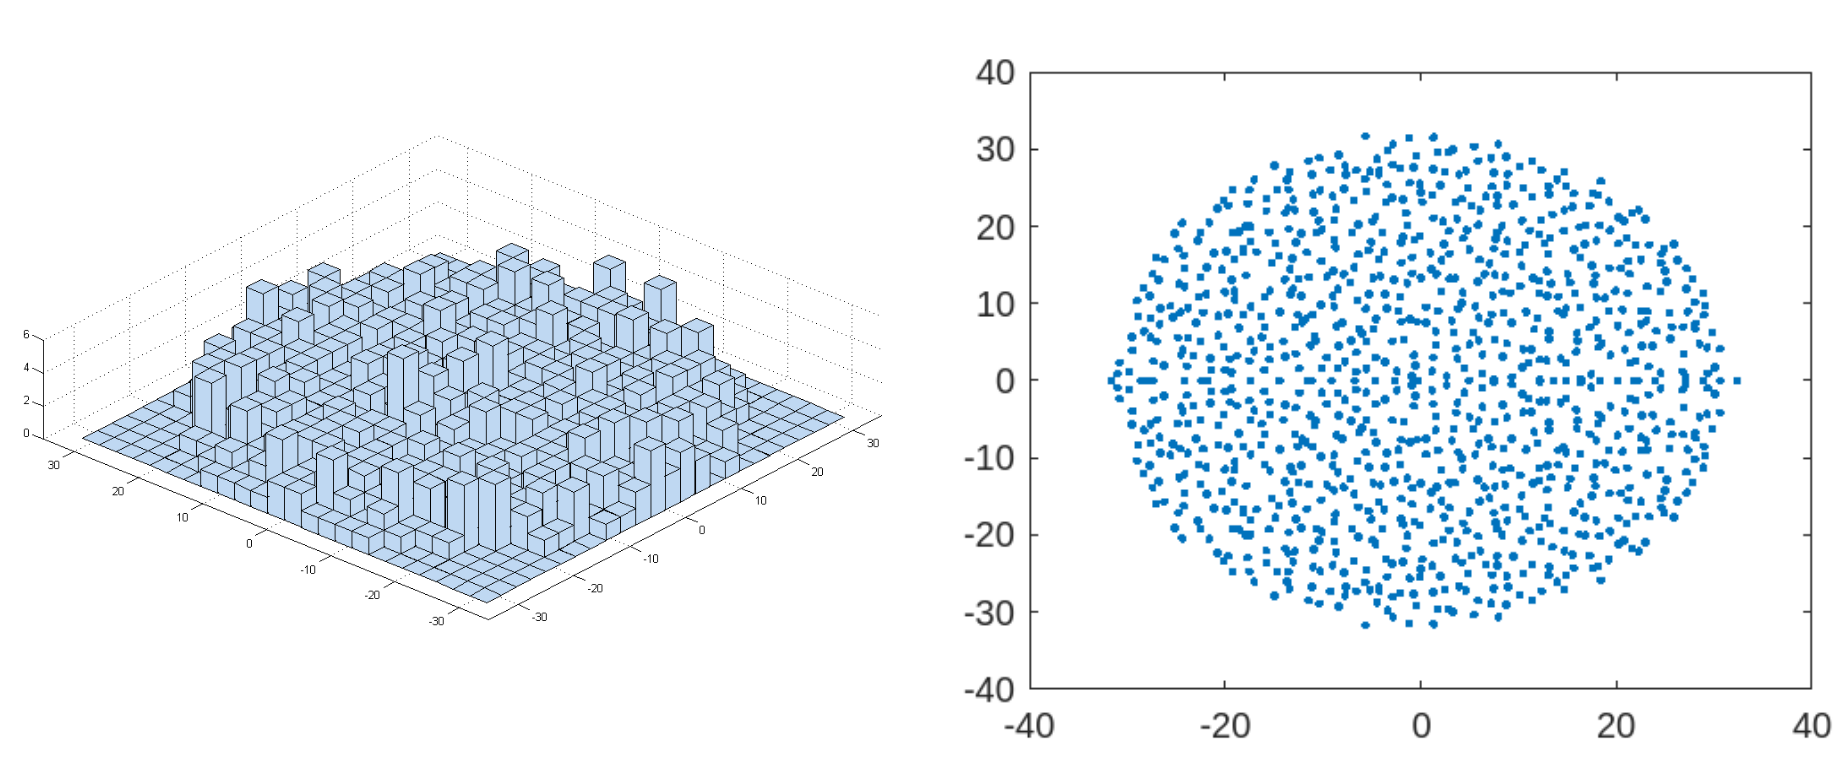
\includegraphics[width=0.9\textwidth]{img/directed_GOE_dist.png}
    \caption{Eigenvalue distribution of a directed GOE random matrix in the complex plane: the eigenvalues are uniformly distributed within a circle of radius \( r = \sigma\sqrt{N} \).}
\end{figure}

To better understand the spectrum of random networks, it is useful to consider the deterministic baseline of regular graphs. In a \textbf{$k$-regular graph}, every node is connected to exactly $k$ neighbors.

\begin{itemize}
    \item \textbf{Principal Eigenvector:} Every $k$-regular graph admits an eigenvector where all components are equal, $\mathbf{v} = (1, 1, \dots, 1)^T$. This highly delocalized vector corresponds exactly to the maximum eigenvalue $\lambda_{max} = k$.
    \item \textbf{Completely Connected Network:} In a fully connected network (or clique), every node is connected to all other nodes, making it a regular graph with $k = N-1$. Its spectrum is highly degenerate: it features a single principal eigenvalue $\lambda_{max} = N-1$, while the remaining $N-1$ eigenvalues are all equal to $-1$. The sum of all eigenvalues (the trace of the adjacency matrix) remains exactly $0$, reflecting the absence of self-loops.
\end{itemize}

\begin{remark}[E-R Spectrum, Wigner Limit, and Disconnected Components]
    In an Erdős-Rényi graph, the expected average degree is $\langle k \rangle = NP$. Because the network behaves macroscopically like a regular graph with this average degree, we observe the isolated principal eigenvalue at $\lambda_{max} \approx NP + 1$.
    Meanwhile, the rest of the eigenvalues $\lambda$ tend toward the Wigner semicircle distribution, representing the random fluctuations around this average connectivity.
\end{remark}

Furthermore, network connectivity directly impacts the zero eigenvalues: if the graph is disconnected (i.e., fragmented into multiple isolated subgraphs), the spectrum of its Laplacian matrix will feature an eigenvalue $\lambda = 0$ with an algebraic multiplicity equal to the exact number of disconnected components.

\begin{figure}[H]
    \begin{minipage}{0.55\textwidth}
        \caption{Eigenvalue distribution of a directed E-R random graph in the complex plane, showing the circular law and the isolated maximum eigenvalue: the eigenvalues are uniformly distributed within a circle of radius \( r = \sigma\sqrt{N} \), while the maximum eigenvalue is located at \( \lambda_{max} \approx NP + 1 \). The presence of the isolated eigenvalue indicates the average connectivity of the graph, while the circular distribution reflects the random nature of the connections.}
    \end{minipage}
    \hfill
    \begin{minipage}{0.4\textwidth}
        \centering
        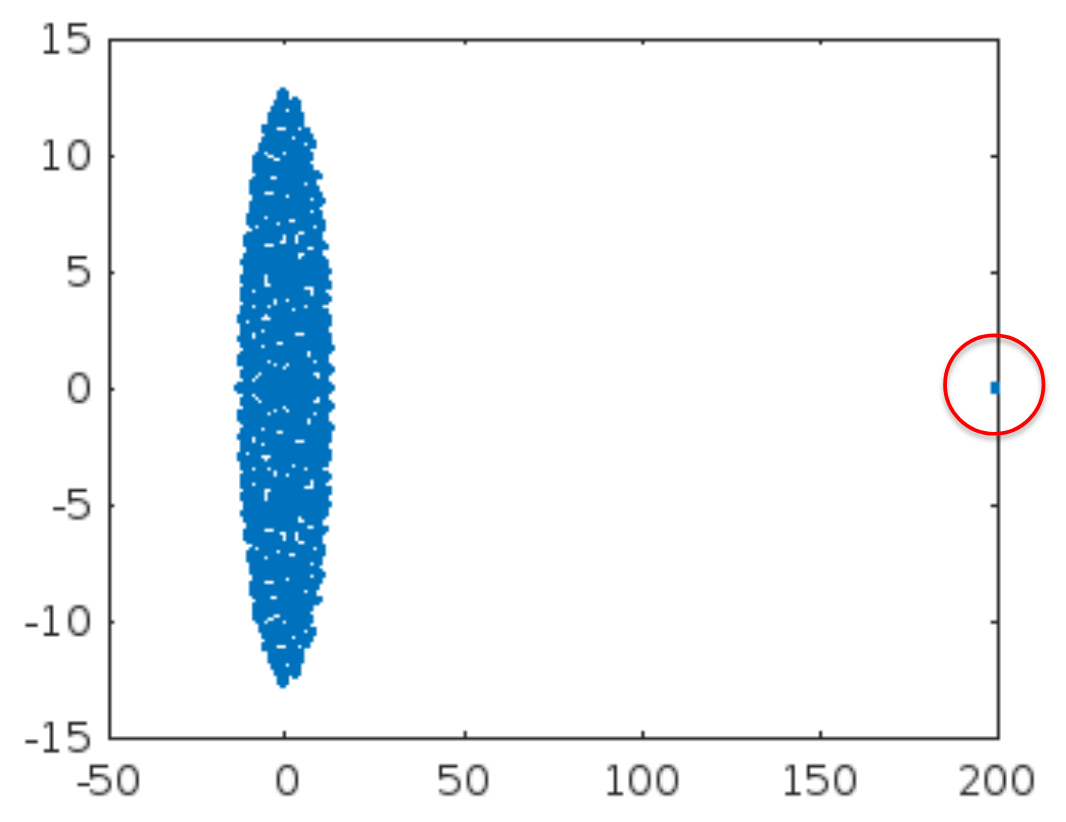
\includegraphics[width=0.9\textwidth]{img/directed_er_dist.png}
    \end{minipage}
\end{figure}

\subsection{Structured Networks: Toeplitz and Circulant Matrices}
While random matrix theory deals with pure topological noise, many real-world networks exhibit strong spatial or deterministic structures that profoundly alter their spectra.

\begin{itemize}
    \item \textbf{Toeplitz Matrices:} In a Toeplitz adjacency matrix, all diagonal bands have constant values: $a_{ij} = f(i-j)$. Physically, this implies that the connection weights between nodes depend solely on their one-dimensional distance. This is a common model for networks sorted along a linear chain, such as polymer backbones or sequential protein structures.
    \item \textbf{Circulant Matrices:} A circulant matrix is a special, highly symmetric case of a Toeplitz matrix where each row is a cyclic shift (modulo $N$) of the preceding row. Topologically, this corresponds to a network with periodic boundary conditions, such as a closed ring lattice. Because of this translational symmetry, the eigenvectors of circulant matrices are independent of the specific matrix elements and can be elegantly solved using the Discrete Fourier Transform.
\end{itemize}

% --------------------------------------------------------
\section{Nearest Neighbor Spacing Distribution (NNSD)}
% --------------------------------------------------------

In addition to the global shape of the spectrum, it is very useful to study the differences between adjacent eigenvalues. Considering the ordered sequence of eigenvalues \( \lambda_1 \le \lambda_2 \le \dots \le \lambda_N \), we define the spacing between two consecutive eigenvalues as \( s_n = \lambda_{n+1} - \lambda_n \).

\begin{definition}[NNSD]
    The Nearest Neighbor Spacing Distribution (NNSD) analyzes the statistical distribution of the spacing ratios \( r_n = \frac{s_{n+1}}{s_n} \). For a matrix belonging to the GOE, this distribution explicitly follows the formula:
    \[ P(r) = \frac{27}{8} \frac{(r+r^2)}{(1+r+r^2)^{5/2}} \]
\end{definition}

This distribution highlights the phenomenon of \textit{level repulsion}: unlike purely random numbers that can cluster freely, the eigenvalues of a random matrix tend to "repel" each other, making it highly improbable to find two identical or very close eigenvalues. This universality property is faithfully preserved even in random E-R graphs.
\begin{figure}[H]
    \centering
    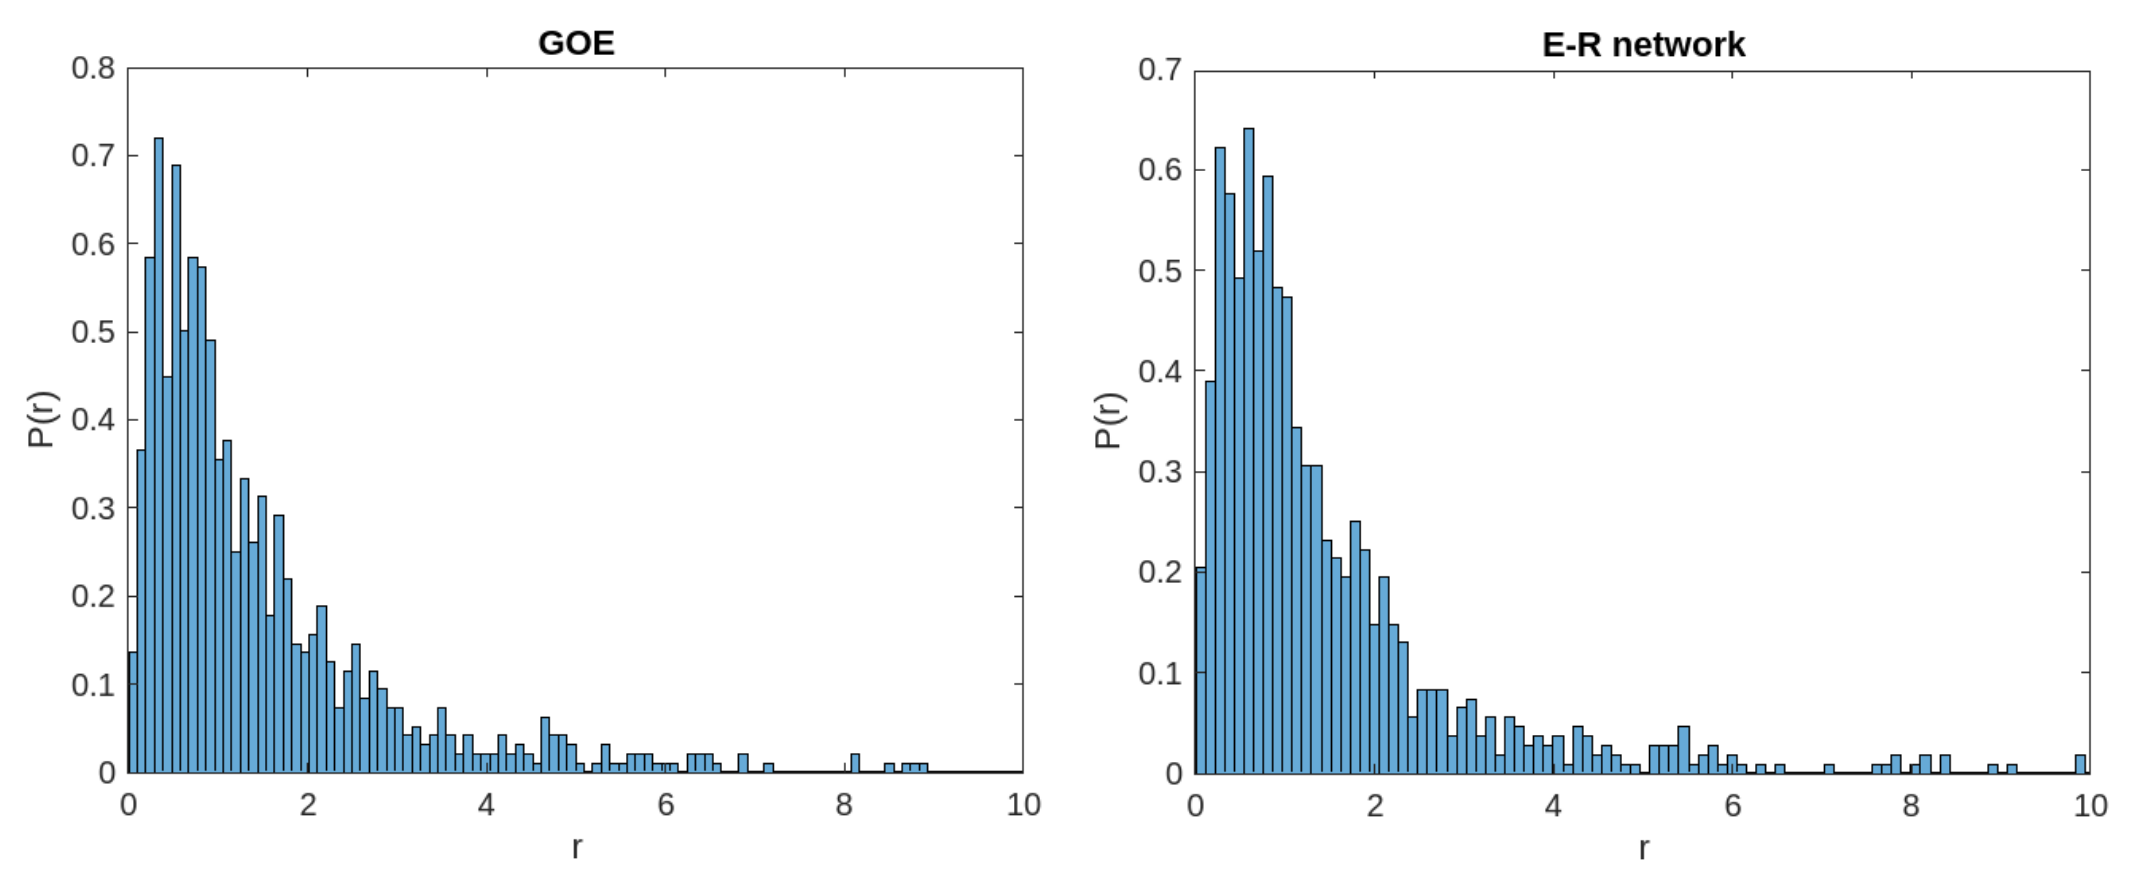
\includegraphics[width=0.9\textwidth]{img/nnsd-goe-er.png}
    \caption{Nearest Neighbor Spacing Distribution (NNSD) for a GOE random matrix and an E-R graph: both follow the same distribution, confirming the universality of level repulsion.}
\end{figure}

\subsection{Biological Application: Hi-C Matrices}

Hi-C is a sophisticated experimental technique used in molecular biology to estimate the spatial proximity of DNA regions within the cell nucleus (3D structure of the genome).
The genome is divided into fragments called "bins" (with typical resolutions of 1 Mb or 100 kb). The experiment generates a large symmetric adjacency matrix, where each element \( A_{ij} \) represents the observed frequency of physical contact between bin \( i \) and bin \( j \).

\begin{figure}[H]
    \begin{minipage}{0.6\textwidth}
        \centering
        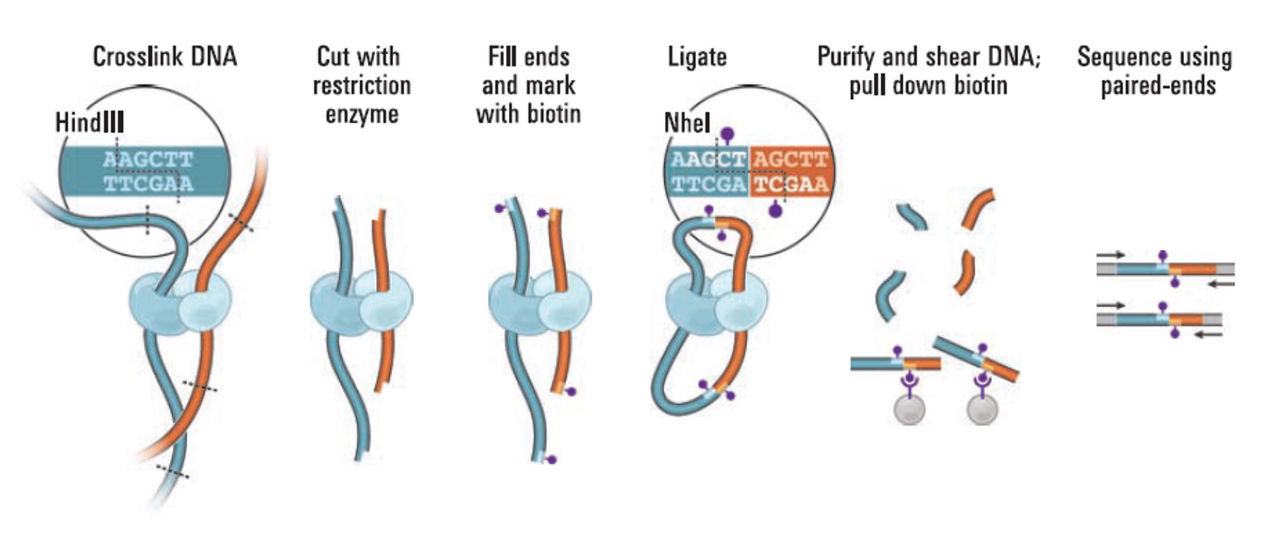
\includegraphics[width=\textwidth]{img/hi-c-experimental_pipeline.png}
    \end{minipage}
    \hfill
    \begin{minipage}{0.35\textwidth}
        \centering
        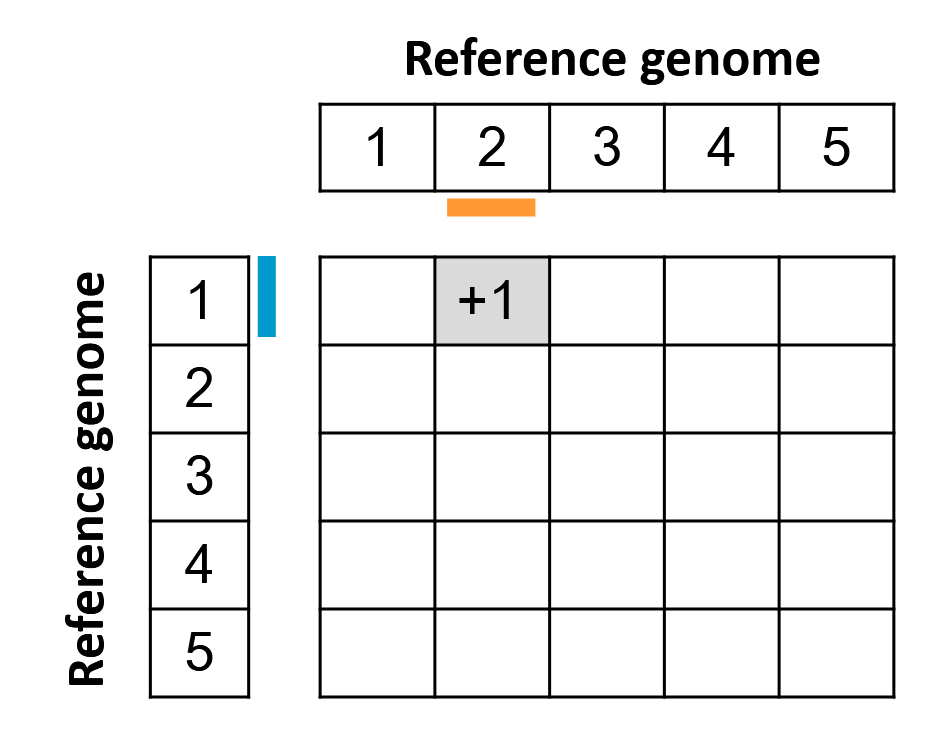
\includegraphics[width=0.9\textwidth]{img/hi-c-matrix.png}
    \end{minipage}
    \caption{Hi-C experimental pipeline and resulting contact matrix: the Hi-C technique generates a large symmetric matrix where each element represents the frequency of physical contact between different regions of the genome. The spectral analysis of this matrix can reveal important insights into the 3D organization of the genome and its functional implications.}
\end{figure}

\subsubsection{Hi-C Spectrum and Noise Filtering (Essential Matrix)}
Applying spectral analysis to a real Hi-C matrix, crucial differences emerge compared to purely random mathematical models:
\begin{itemize}
    \item \textbf{Eigenvalues}: A central "bulk" is observed that follows GOE rules (representing the pure background noise of the experiment) and a pronounced tail of isolated eigenvalues that contain the true structural biological "signal".
    \item \textbf{Eigenvectors}: Unlike the purely Gaussian components of the GOE, the eigenvectors corresponding to the signal eigenvalues show heavy tails. This indicates that they carry differentiated and highly localized biological information, useful for identifying topologically associating domains (TADs).
\end{itemize}

\begin{figure}[H]
    \begin{minipage}{0.55\textwidth}
        \begin{minipage}{\linewidth}
            \centering
            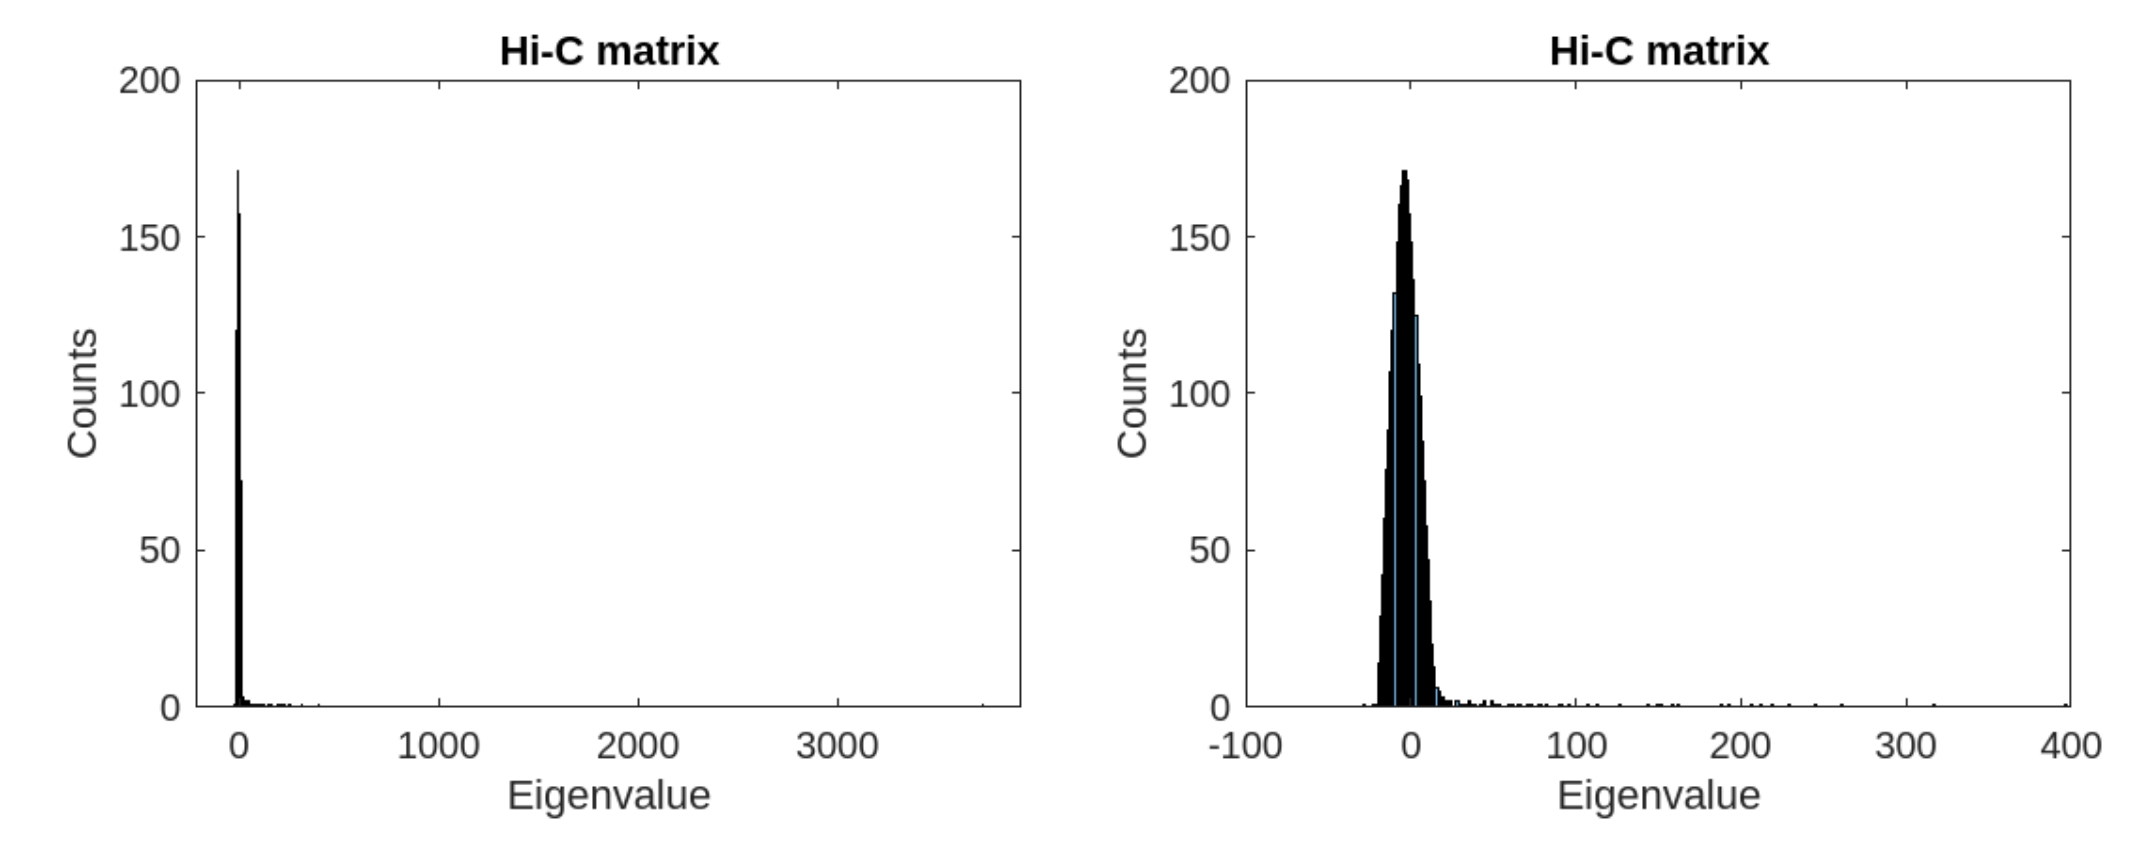
\includegraphics[width=0.9\textwidth]{img/hi-c-spectrum_noise.png}
        \end{minipage}
        \vspace{0.5cm}
        \begin{minipage}{\linewidth}
            \centering
            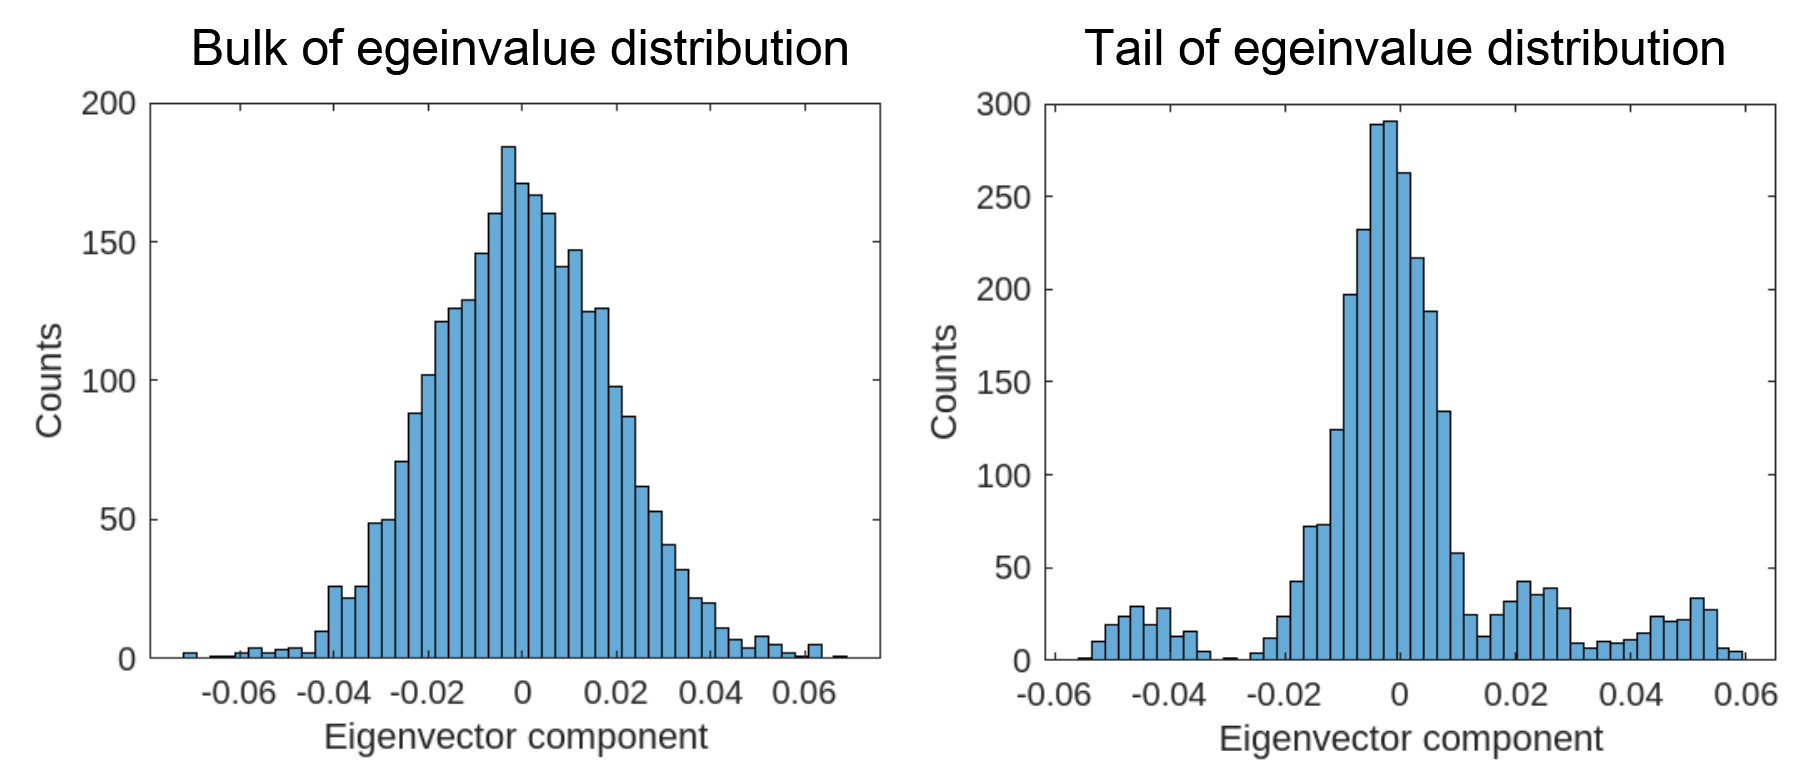
\includegraphics[width=0.9\textwidth]{img/hi-c-eigenvec_dist.png}
        \end{minipage}
    \end{minipage}
    \hfill
    \begin{minipage}{0.4\textwidth}
        \caption{Hi-C spectrum and eigenvector distribution: the spectrum of a real Hi-C matrix shows a clear separation between a central bulk (noise) and isolated eigenvalues (signal). The eigenvectors corresponding to the signal eigenvalues exhibit heavy-tailed distributions, indicating that they carry localized biological information.}
    \end{minipage}
\end{figure}

By exploiting this clear separation between noise (the bulk) and structural information (the outliers), it is possible to clean the data by reconstructing an \textbf{Essential Hi-C Matrix}. Similar to Principal Component Analysis (PCA), the original network is projected only onto the first \( n^* \) principal eigenvectors that carry the real signal:
\[ A_{ij}^{ess} = \sum_{n=1}^{n^*} \lambda_n a_n^{(i)} a_n^{(j)} \]

\begin{figure}[H]
    \begin{minipage}{0.5\textwidth}
        \caption{The essential Hi-C matrix in comparison to the original one:...}
    \end{minipage}
    \hfill
    \begin{minipage}{0.45\textwidth}
        \centering
        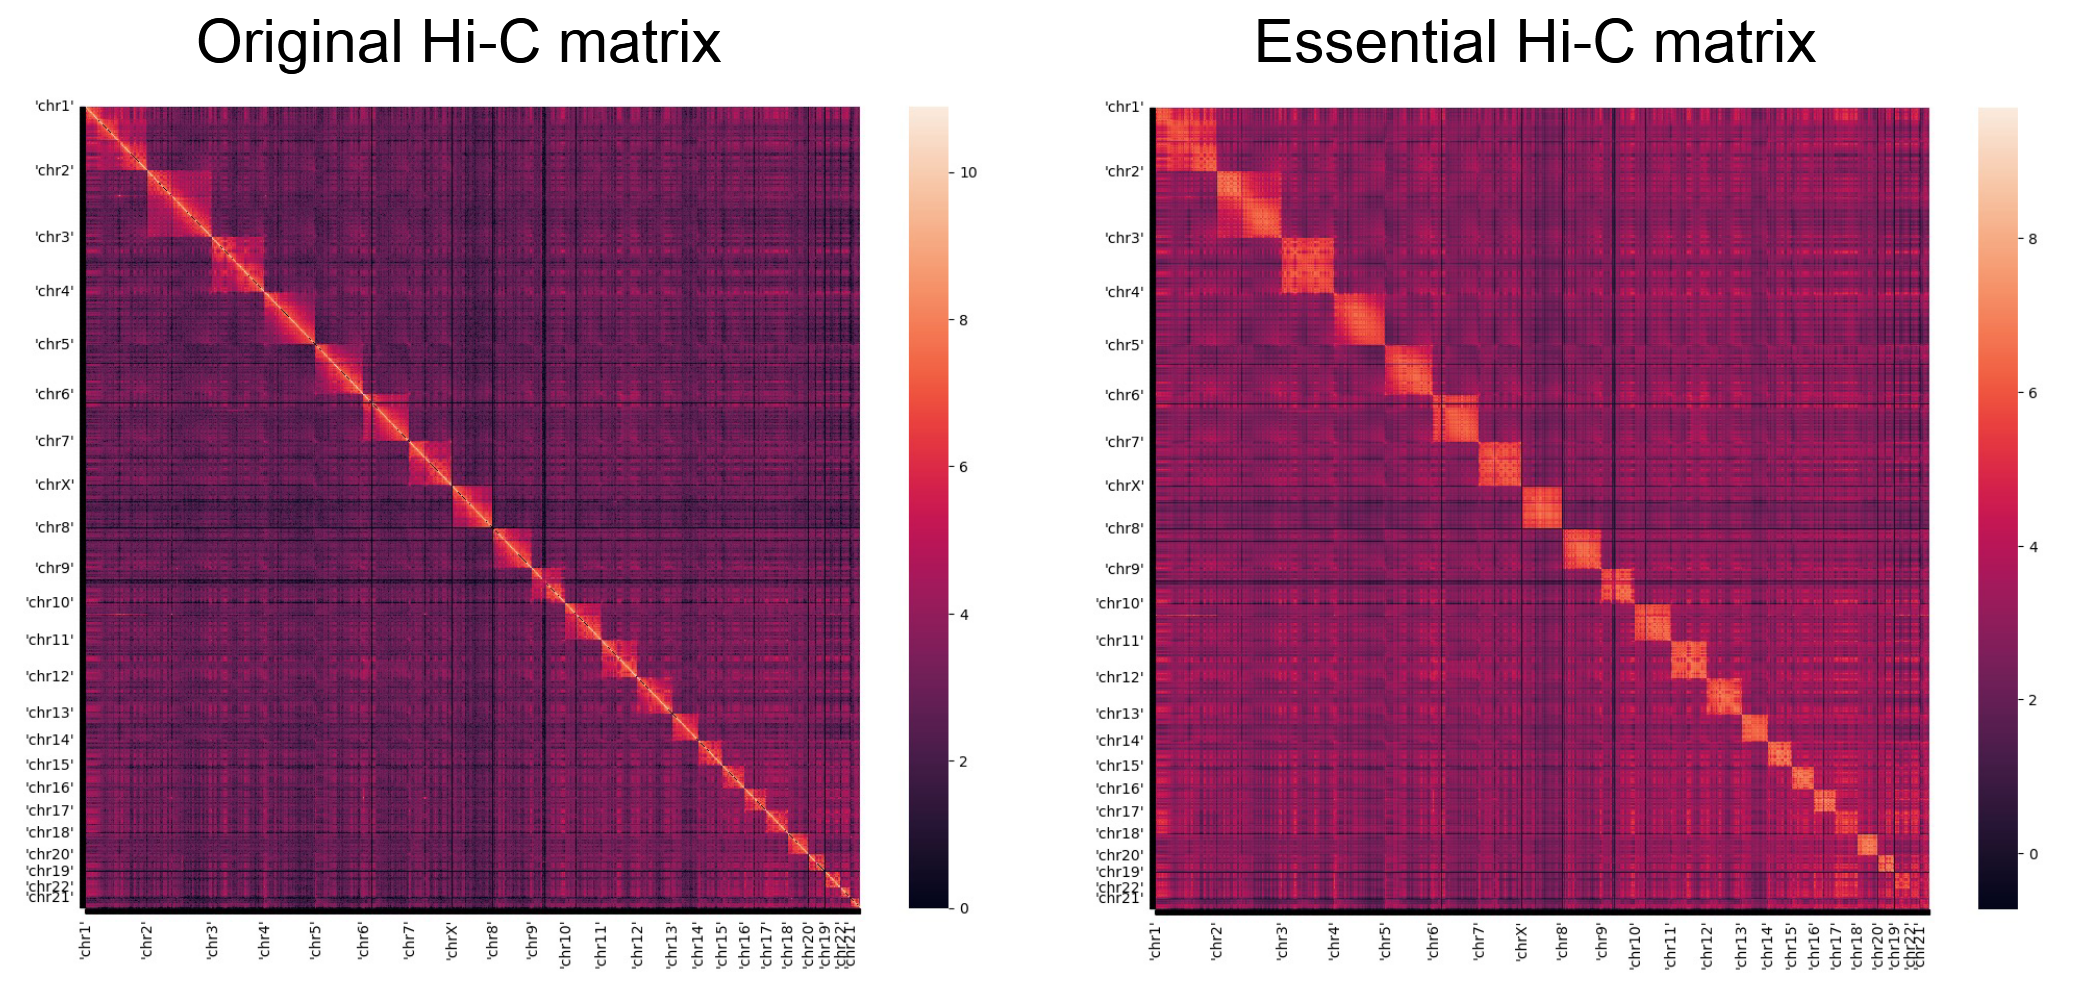
\includegraphics[width=0.9\textwidth]{img/essential_hi-c.png}
    \end{minipage}
\end{figure}

Finally we can compare the NNSD for the Hi-C matrix with the GOE distribution. This tells us about only the short-range correlations in eigenvalues, thus capturing the universality present in a wide range of complex networks.

\begin{figure}[H]
    \begin{minipage}{0.5\textwidth}
        \centering
        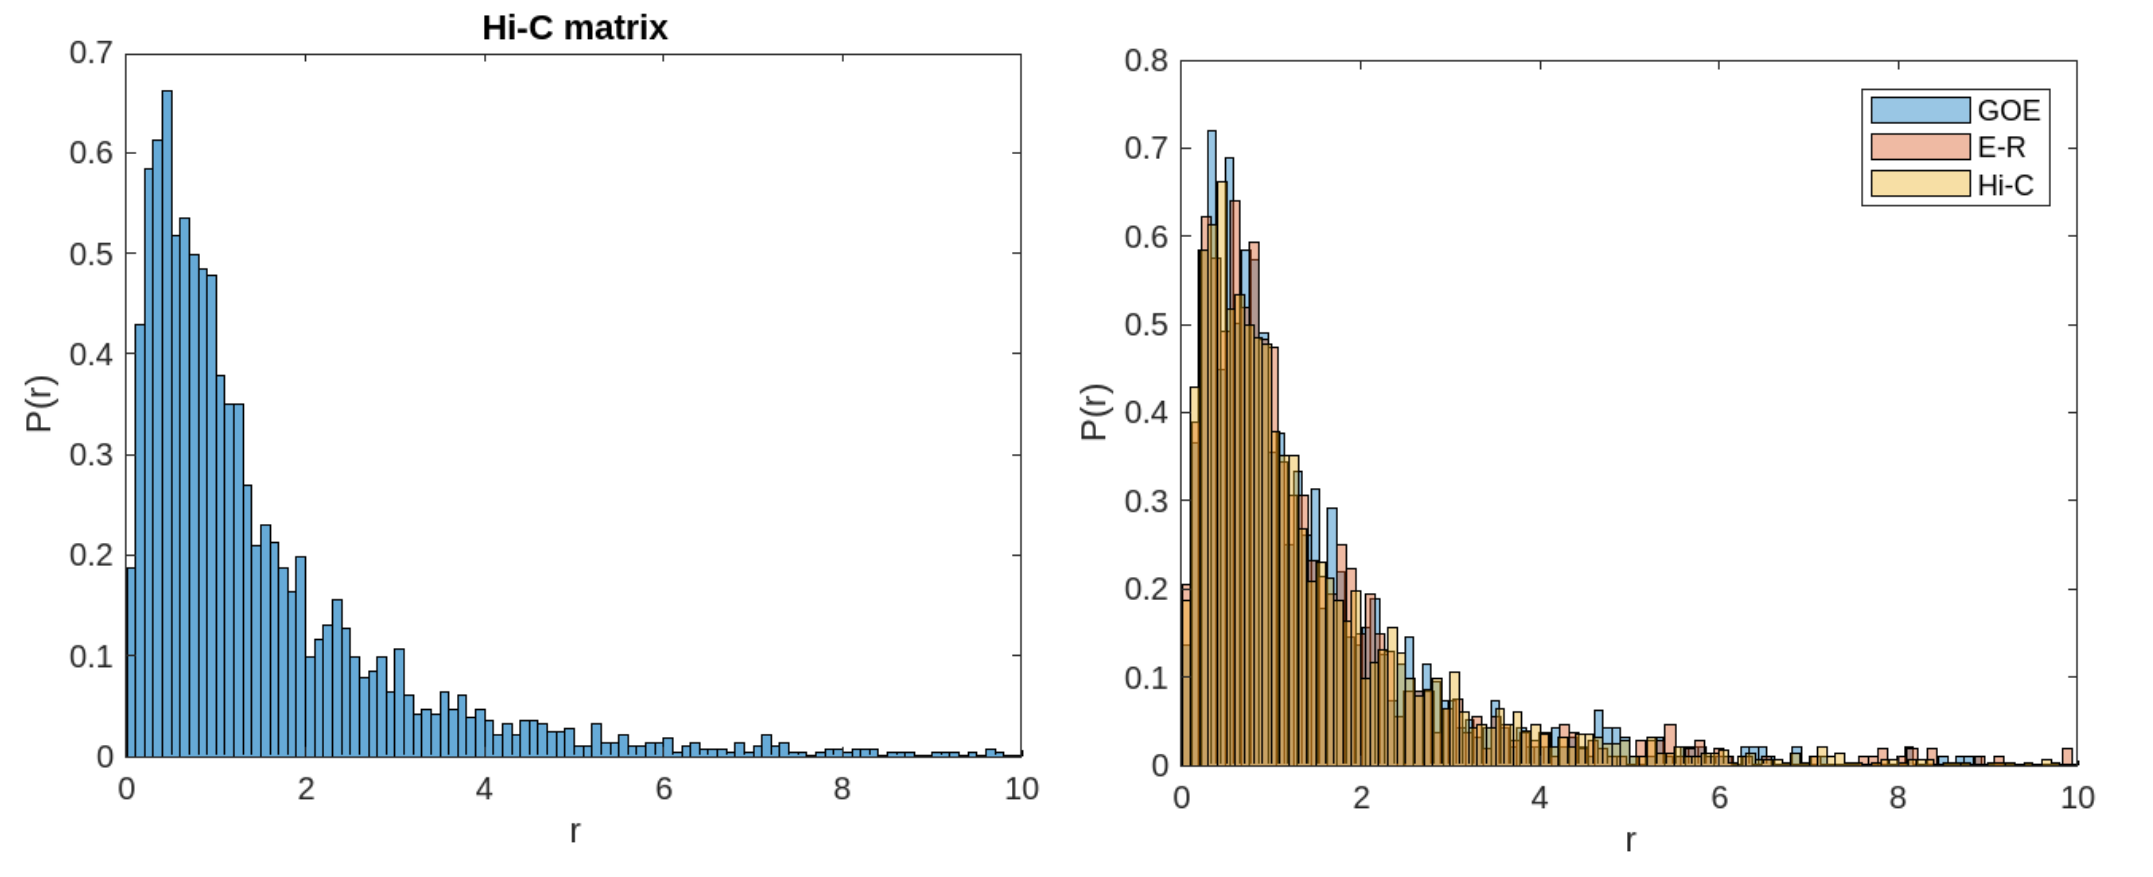
\includegraphics[width=0.9\textwidth]{img/nnsd-hi-c_goe_er.png}
    \end{minipage}
    \hfill
    \begin{minipage}{0.45\textwidth}
        \caption{Comparison...}
    \end{minipage}
\end{figure}

% --------------------------------------------------------
\section{Free Probability Theory and the Laplacian}
% --------------------------------------------------------

\subsection{Generalization of the Semicircle}
The strength of the semicircle law lies in its robustness: it applies not only to matrices with Gaussian elements but also to matrices where the weights are drawn from arbitrary distributions, provided they are independent and have finite variance. This concept is the basis of the Central Limit Theorem for matrices. Furthermore, the spectrum resulting from the sum of two independent ("free") random matrices can be elegantly calculated using the so-called "free convolution" of their individual spectra.

\subsection{Covariance Matrices and the Spectrum of the Laplacian}
Covariance matrices generated from random data do not follow the semicircle law, but rather the renowned \textbf{Marchenko-Pastur} eigenvalue distribution.
Since the Laplacian matrix \( L \) of a random directed graph can be factorized as the product of the incidence matrix \( I \) and its transpose (\( L = I^T I \)), its algebraic structure is similar to that of a covariance matrix. Consequently, the eigenvalue spectrum of the Laplacian of an E-R graph is directly modeled by the Marchenko-Pastur distribution.

\begin{figure}[H]
    \begin{minipage}{0.5\textwidth}
        \centering
        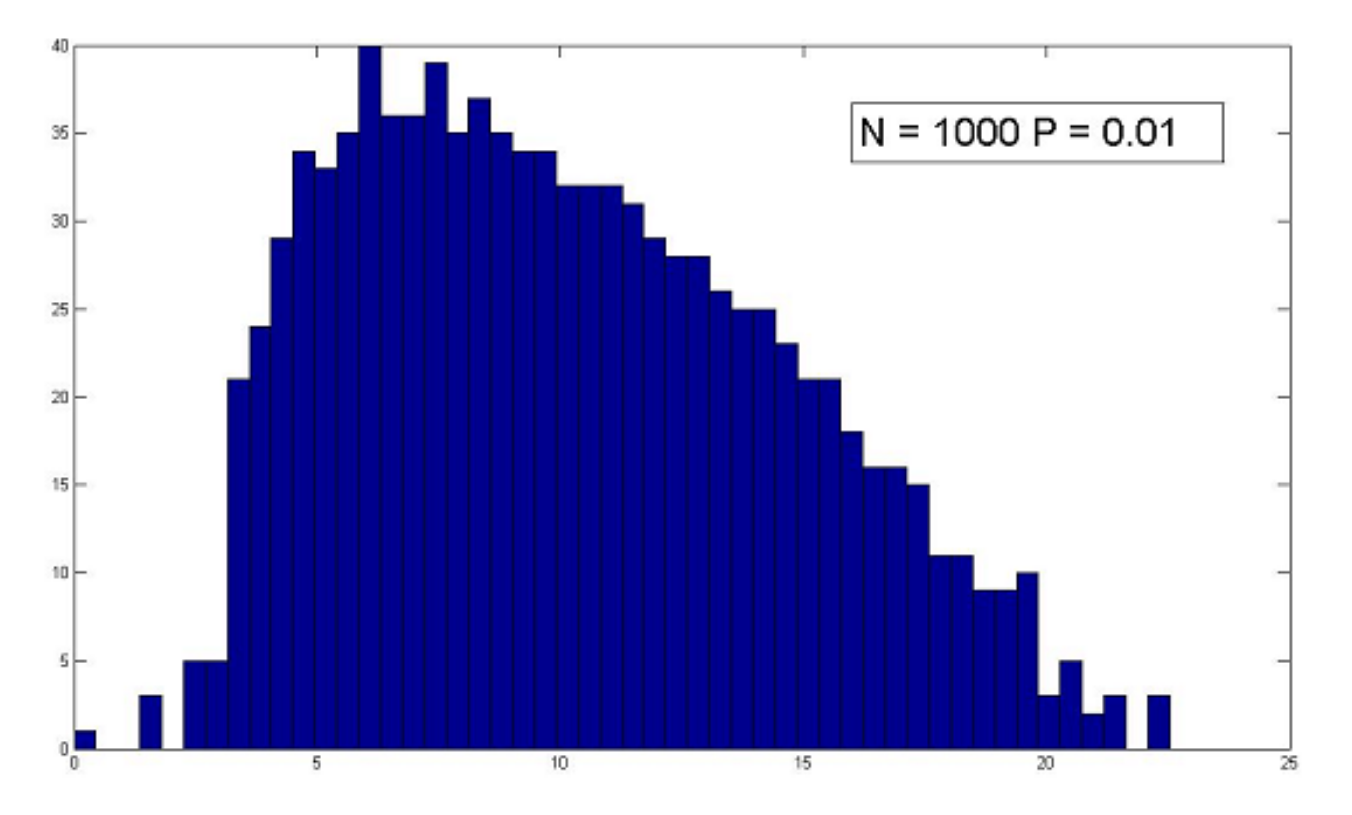
\includegraphics[width=0.9\textwidth]{img/marcenko-pastur-dist.png}
    \end{minipage}
    \hfill
    \begin{minipage}{0.45\textwidth}
        \caption{ooooooooooo}
    \end{minipage}
\end{figure}

\begin{remark}[Participation Ratio]
    To rigorously quantify whether the components of an eigenvector are homogeneous (delocalized) or concentrated on a few specific nodes (localized), the \textbf{Participation Ratio (PR)} is calculated.
    Given a normalized eigenvector where \( \sum v_i^2 = 1 \), the PR is defined as:
    \[ PR = \sum_{i=1}^N v_i^4 \]
    The conceptual limits of this metric are:
    \begin{itemize}
        \item \( PR \to \frac{1}{N} \): The eigenvector is perfectly delocalized (e.g., a completely uniform network where all nodes have equal weight).
        \item \( PR \to 1 \): The eigenvector is totally localized (all information is concentrated on a single node).
    \end{itemize}
    In E-R networks, the eigenvectors of the Laplacian exhibit "heavy" tails. However, even though they are not Gaussian, the PR values remain statistically homogeneous across the various eigenvectors, confirming the absence of dominant hubs and the substantial topological indistinguishability of nodes in the Erdős-Rényi model.
\end{remark}